\chapter{Method}

\begin{figure}[H]
	\centering
	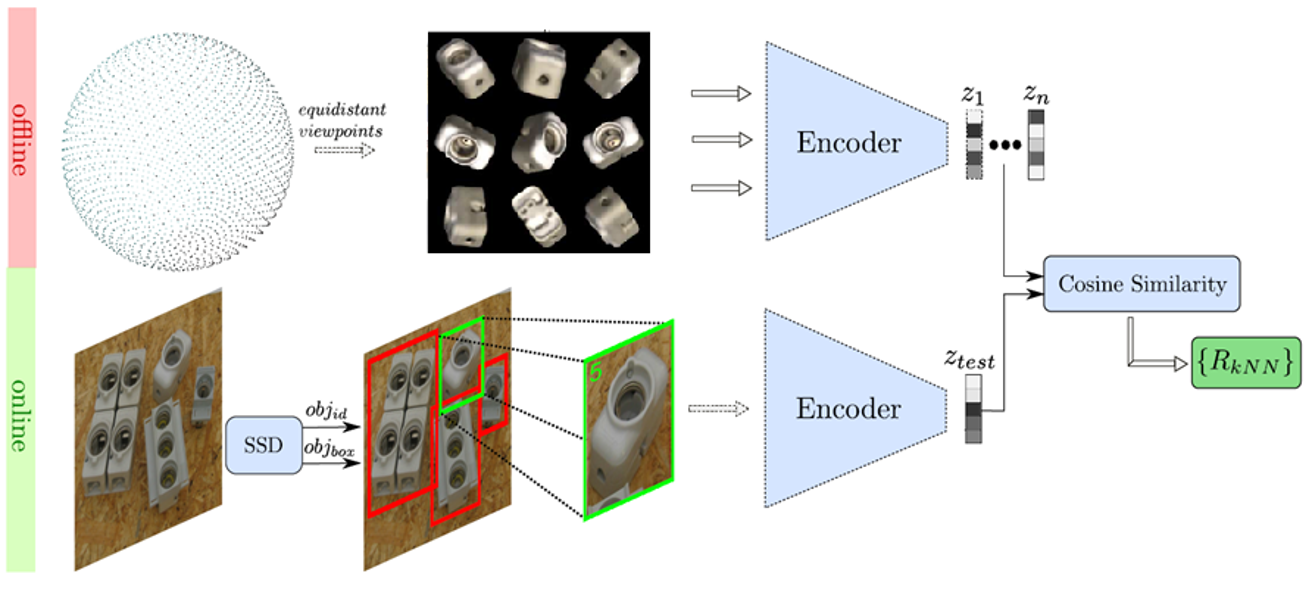
\includegraphics[width=0.9\textwidth]{structure}
	\caption[Object pose estimation pipeline]{\textbf{Object pose estimation pipeline}}
	\label{fig:structure}
\end{figure}

The main idea of this approach is to implicitly learn representations from rendered 3d model views with autoencoder, and then determine the orientation of the object employing the nearest neighbor search. On one hand, since it avoids one-to-many mappings from images to orientations, it is able to handle ambiguous poses caused by symmetric views. In another hand, it can be trained on synthetic object views in a self-supervised way and hence removes the need for a large pose-annotated dataset. Besides, by applying random augmentations on the training dataset, it is able to yield a robust estimation against occlusion and cluttered backgrounds.  \\[8pt]
The pose estimation pipeline can be divided into two parts: an offline part and an online part. In the offline part, an autoencoder is trained on the synthetic dataset, and then a codebook is created by encoding the dataset. At test time, the pose of the object is estimated using the nearest neighbor search with the highest cosine similarity from the codebook. However, due to time constraints, the object detection will not be implemented in my project.  \\[8pt]






\section{Synthetic Dataset Creation}

Since simply sampling points with permissible intervals in spherical coordinates will not result in an evenly placed points on the sphere surface, I sample viewpoints using Fibonacci Lattice as suggested in \cite{deserno2004generate}. In this sampling approach, points in the unit square $[0,\,1]$ will be first mapped to spherical coordinates with \eqref{eq:sample1}, and then be converted to euclidean coordinate using \eqref{eq:sample2}. The uniform sampling results are demonstrated in Fig. \ref{fig:uniformsample}. Fig. \ref{fig:regular} shows the regularly sampled points, while Fig. \ref{fig:random} the randomly sampled points.
  
\begin{align}
(x,\,y) \rightarrow (\theta,\, \phi) : (cos^{-1}(2x-1)-\pi /2, \, 2\pi y)
\label{eq:sample1} 
\\
(\theta,\, \phi) \rightarrow (x, \, y, \, z) : (cos \theta \, cos\phi, \, cos\theta \, sin\phi,sin \theta )
\label{eq:sample2} 
\end{align}

\begin{figure}[H]
	\centering
	\subfigure[regular sampling]{
		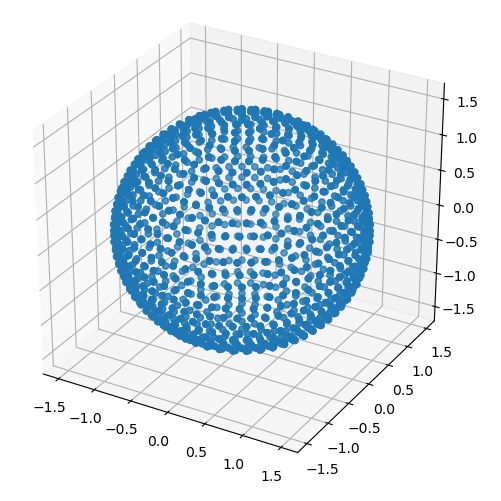
\includegraphics[width=0.4\textwidth] {uniformsampling}
		\label{fig:regular}
	}
	\qquad 
	\subfigure[random sampling]{
		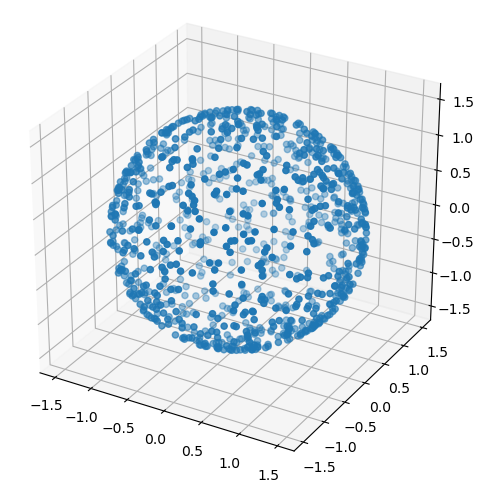
\includegraphics[width=0.4\textwidth] {randomsampling}
		\label{fig:random}
	}
	\caption[Uniform sampling of the synthetic object viewpoints]{\textbf{Uniform sampling of the synthetic object viewpoints} }
	\label{fig:uniformsample}
\end{figure}


\section{Autoencoder Training}
In order to generalize from synthetic to real data, random augmentations are applied on the rendered dataset to simulate variant real environments, and the autoencoder is trained to best reconstruct the target images from the augmented input images. The training process is illustrated in Fig. \ref{fig:autoencoder}. Fig. \ref{fig:newautoencoder} illustrates the convolutional architecture of the autoencoder used in the project, and the per-sample loss is the sum over the pixel-wise L2 distance as described in Eq. \ref{eq:loss}]. 

\begin{align}
	l_2 = \sum_{i \in \mathcal{D} } || x_{(i)}-\hat{x}_{(i)} || _2
	\label{eq:loss}
\end{align}


\begin{figure}[H]
	\centering
	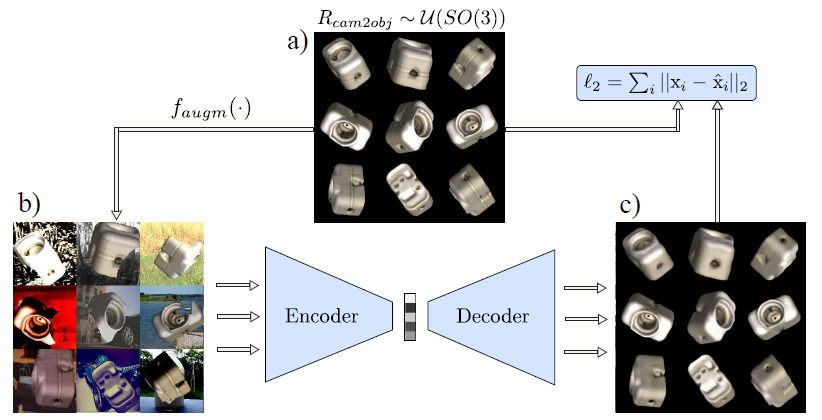
\includegraphics[width=0.8\textwidth]{autoencoder}
	\caption[Training process of the autoencoder]{\textbf{Training process of the autoencoder.} a) Reconstruction target, b) augmented input image, c) reconstructed image.}
	\label{fig:autoencoder}
\end{figure}
\begin{figure}[H]
	\centering
	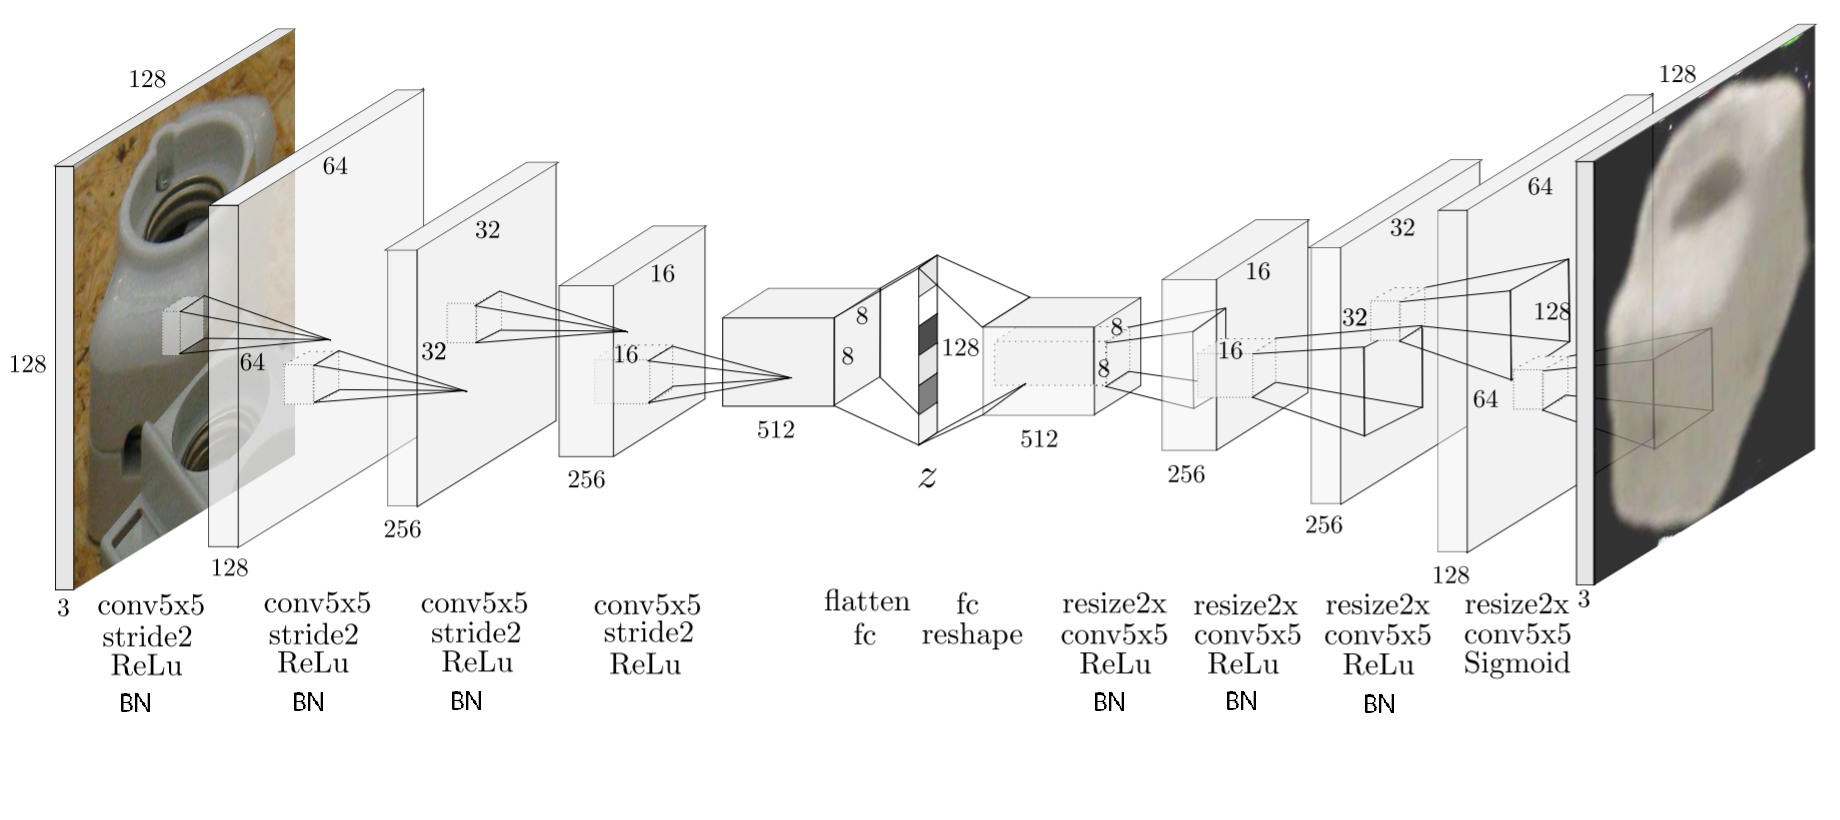
\includegraphics[width=1\textwidth]{newautoencoder}
	\caption[Autoencoder architecture]{\textbf{Autoencoder architecture}}
	\label{fig:newautoencoder}
\end{figure}


After the training, the autoencoder is able to extract the object from real scene crops, while the clarity and the orientation of the decoder reconstruction indicates the encoding quality. 

\section{3D Pose Estimation}
To determine the object orientation, a codebook is firstly created at the offline stage, which contains the latent encodings $z_i \in \mathcal{R}^{128} $ of object views at equidistant viewpoints from a full view-sphere. 
 \\[8pt]
 At test time, the image crops of the considered objects will be resized and forwarded to the encoder network. After encoding, the highest cosine similarity between the test code $z_{test} \in \mathcal{R}^{128}$ and all codes from the codebook will be searched via the nearest neighbor algorithm, and the corresponding rotation matrix will be determined as the object orientation.  
\begin{align}
cos_i = \frac{z_i \, z_{test}}{||z_i||\, ||z_{test}||}
\label{eq:cosineloss} 
\end{align}